\documentclass{standalone}
\usepackage{tikz}
\usetikzlibrary{patterns, positioning}


\begin{document}
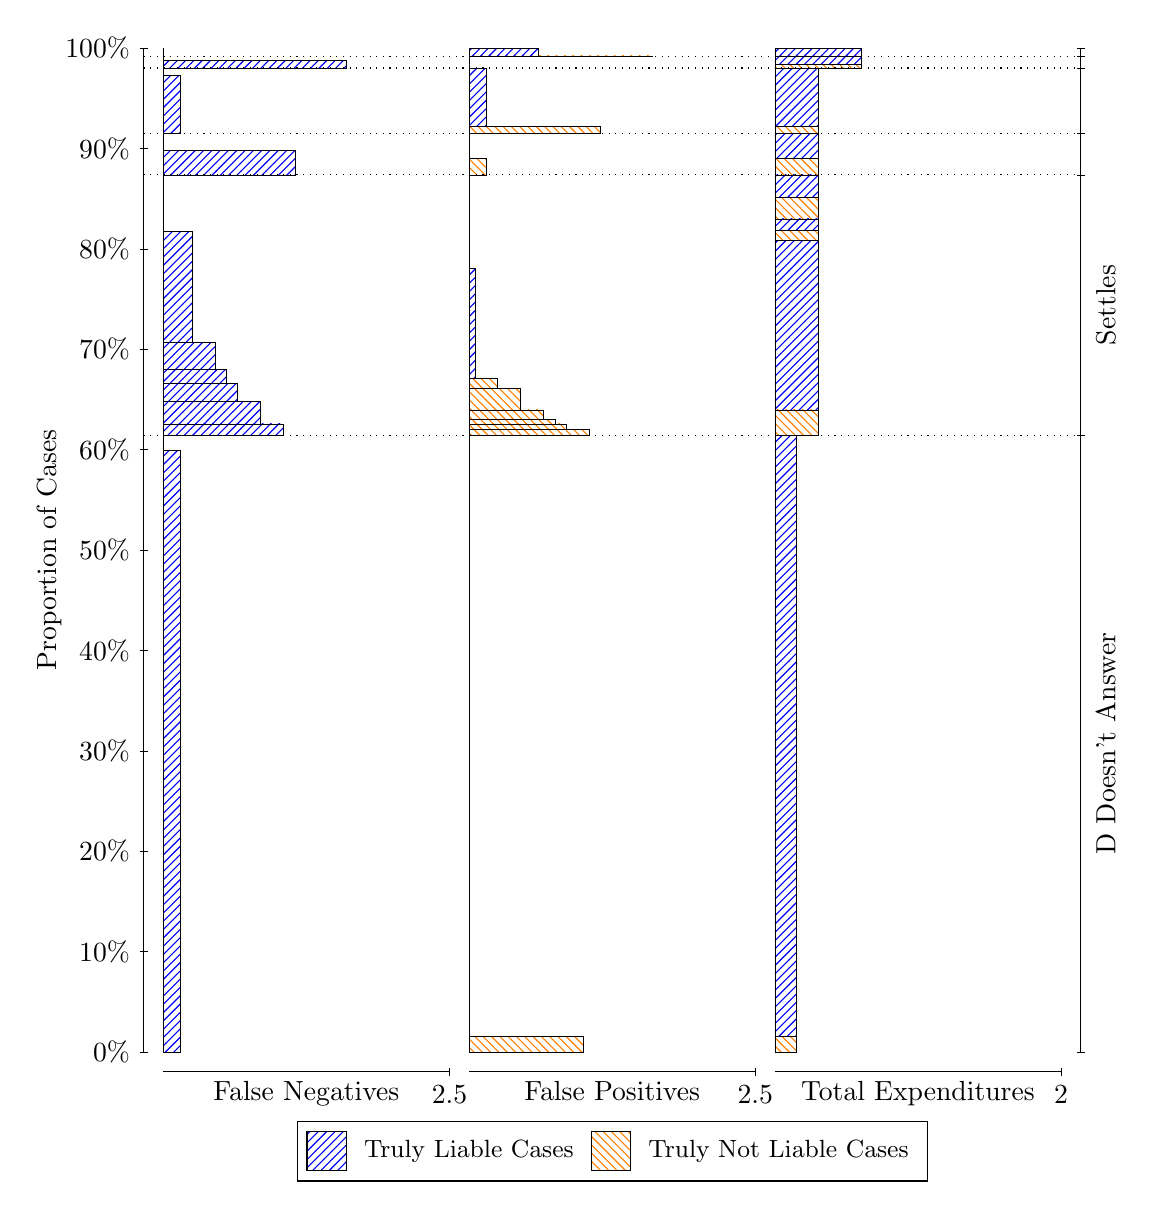
\begin{tikzpicture}
\draw[black, very thin] (1.5,1.75) -- (1.5,14.5);
\node[rotate=90, text=black, anchor=center] at (0.3, 8.125) {Proportion of Cases};
\draw[black, very thin] (1.45,1.75) -- (1.55,1.75);
\node[text=black, anchor=east] at (1.45, 1.75) {0\%};
\draw[black, very thin] (1.45,3.025) -- (1.55,3.025);
\node[text=black, anchor=east] at (1.45, 3.025) {10\%};
\draw[black, very thin] (1.45,4.3) -- (1.55,4.3);
\node[text=black, anchor=east] at (1.45, 4.3) {20\%};
\draw[black, very thin] (1.45,5.575) -- (1.55,5.575);
\node[text=black, anchor=east] at (1.45, 5.575) {30\%};
\draw[black, very thin] (1.45,6.85) -- (1.55,6.85);
\node[text=black, anchor=east] at (1.45, 6.85) {40\%};
\draw[black, very thin] (1.45,8.125) -- (1.55,8.125);
\node[text=black, anchor=east] at (1.45, 8.125) {50\%};
\draw[black, very thin] (1.45,9.4) -- (1.55,9.4);
\node[text=black, anchor=east] at (1.45, 9.4) {60\%};
\draw[black, very thin] (1.45,10.675) -- (1.55,10.675);
\node[text=black, anchor=east] at (1.45, 10.675) {70\%};
\draw[black, very thin] (1.45,11.95) -- (1.55,11.95);
\node[text=black, anchor=east] at (1.45, 11.95) {80\%};
\draw[black, very thin] (1.45,13.225) -- (1.55,13.225);
\node[text=black, anchor=east] at (1.45, 13.225) {90\%};
\draw[black, very thin] (1.45,14.5) -- (1.55,14.5);
\node[text=black, anchor=east] at (1.45, 14.5) {100\%};

\draw[black, very thin] (13.4,1.75) -- (13.4,14.5);
\draw[black, very thin] (13.35,1.75) -- (13.45,1.75);
\node[anchor=west] at (13.35, 1.75) {};
\draw[black, very thin] (13.35,9.5828) -- (13.45,9.5828);
\node[anchor=west] at (13.35, 9.5828) {};
\draw[black, very thin] (13.35,12.889) -- (13.45,12.889);
\node[anchor=west] at (13.35, 12.889) {};
\draw[black, very thin] (13.35,13.413) -- (13.45,13.413);
\node[anchor=west] at (13.35, 13.413) {};
\draw[black, very thin] (13.35,14.246) -- (13.45,14.246);
\node[anchor=west] at (13.35, 14.246) {};
\draw[black, very thin] (13.35,14.389) -- (13.45,14.389);
\node[anchor=west] at (13.35, 14.389) {};
\draw[black, very thin] (13.35,14.5) -- (13.45,14.5);
\node[anchor=west] at (13.35, 14.5) {};

\draw[black, very thin, pattern color=blue, pattern=north east lines] (1.75,1.75) rectangle (1.968,9.3892);
\draw[black, very thin, pattern color=orange, pattern=north west lines] (1.75,9.3892) rectangle (1.75,9.5828);
\draw[black, very thin, pattern color=blue, pattern=north east lines] (1.75,9.5828) rectangle (3.276,9.7279);
\draw[black, very thin, pattern color=blue, pattern=north east lines] (1.75,9.7279) rectangle (2.9853,10.016);
\draw[black, very thin, pattern color=blue, pattern=north east lines] (1.75,10.016) rectangle (2.6947,10.243);
\draw[black, very thin, pattern color=blue, pattern=north east lines] (1.75,10.243) rectangle (2.5493,10.421);
\draw[black, very thin, pattern color=blue, pattern=north east lines] (1.75,10.421) rectangle (2.404,10.762);
\draw[black, very thin, pattern color=blue, pattern=north east lines] (1.75,10.762) rectangle (2.1133,12.167);
\draw[black, very thin, pattern color=orange, pattern=north west lines] (1.75,12.167) rectangle (1.75,12.889);
\draw[black, very thin, pattern color=blue, pattern=north east lines] (1.75,12.889) rectangle (3.4213,13.202);
\draw[black, very thin, pattern color=orange, pattern=north west lines] (1.75,13.202) rectangle (1.75,13.413);
\draw[black, very thin, pattern color=blue, pattern=north east lines] (1.75,13.413) rectangle (1.968,14.153);
\draw[black, very thin, pattern color=orange, pattern=north west lines] (1.75,14.153) rectangle (1.75,14.246);
\draw[black, very thin, pattern color=blue, pattern=north east lines] (1.75,14.246) rectangle (4.0753,14.345);
\draw[black, very thin, pattern color=orange, pattern=north west lines] (1.75,14.345) rectangle (1.75,14.389);
\draw[black, very thin, pattern color=orange, pattern=north west lines] (1.75,14.389) rectangle (1.75,14.4);
\draw[black, very thin, pattern color=blue, pattern=north east lines] (1.75,14.4) rectangle (1.75,14.5);
\draw[black, very thin, pattern color=orange, pattern=north west lines] (5.6333,1.75) rectangle (7.0867,1.9437);
\draw[black, very thin, pattern color=blue, pattern=north east lines] (5.6333,1.9437) rectangle (5.6333,9.5828);
\draw[black, very thin, pattern color=orange, pattern=north west lines] (5.6333,9.5828) rectangle (7.1593,9.6591);
\draw[black, very thin, pattern color=orange, pattern=north west lines] (5.6333,9.6591) rectangle (6.8687,9.7259);
\draw[black, very thin, pattern color=orange, pattern=north west lines] (5.6333,9.7259) rectangle (6.7233,9.7821);
\draw[black, very thin, pattern color=orange, pattern=north west lines] (5.6333,9.7821) rectangle (6.578,9.9048);
\draw[black, very thin, pattern color=orange, pattern=north west lines] (5.6333,9.9048) rectangle (6.2873,10.175);
\draw[black, very thin, pattern color=orange, pattern=north west lines] (5.6333,10.175) rectangle (5.9967,10.304);
\draw[black, very thin, pattern color=blue, pattern=north east lines] (5.6333,10.304) rectangle (5.706,11.709);
\draw[black, very thin, pattern color=blue, pattern=north east lines] (5.6333,11.709) rectangle (5.6333,12.889);
\draw[black, very thin, pattern color=orange, pattern=north west lines] (5.6333,12.889) rectangle (5.8513,13.1);
\draw[black, very thin, pattern color=blue, pattern=north east lines] (5.6333,13.1) rectangle (5.6333,13.413);
\draw[black, very thin, pattern color=orange, pattern=north west lines] (5.6333,13.413) rectangle (7.3047,13.507);
\draw[black, very thin, pattern color=blue, pattern=north east lines] (5.6333,13.507) rectangle (5.8513,14.246);
\draw[black, very thin, pattern color=orange, pattern=north west lines] (5.6333,14.246) rectangle (5.6333,14.291);
\draw[black, very thin, pattern color=blue, pattern=north east lines] (5.6333,14.291) rectangle (5.6333,14.389);
\draw[black, very thin, pattern color=orange, pattern=north west lines] (5.6333,14.389) rectangle (7.9587,14.4);
\draw[black, very thin, pattern color=blue, pattern=north east lines] (5.6333,14.4) rectangle (6.5053,14.5);
\draw[black, very thin, pattern color=orange, pattern=north west lines] (9.5167,1.75) rectangle (9.7892,1.9437);
\draw[black, very thin, pattern color=blue, pattern=north east lines] (9.5167,1.9437) rectangle (9.7892,9.5828);
\draw[black, very thin, pattern color=orange, pattern=north west lines] (9.5167,9.5828) rectangle (10.062,9.9048);
\draw[black, very thin, pattern color=blue, pattern=north east lines] (9.5167,9.9048) rectangle (10.062,12.056);
\draw[black, very thin, pattern color=orange, pattern=north west lines] (9.5167,12.056) rectangle (10.062,12.185);
\draw[black, very thin, pattern color=blue, pattern=north east lines] (9.5167,12.185) rectangle (10.062,12.33);
\draw[black, very thin, pattern color=orange, pattern=north west lines] (9.5167,12.33) rectangle (10.062,12.6);
\draw[black, very thin, pattern color=blue, pattern=north east lines] (9.5167,12.6) rectangle (10.062,12.889);
\draw[black, very thin, pattern color=orange, pattern=north west lines] (9.5167,12.889) rectangle (10.062,13.1);
\draw[black, very thin, pattern color=blue, pattern=north east lines] (9.5167,13.1) rectangle (10.062,13.413);
\draw[black, very thin, pattern color=orange, pattern=north west lines] (9.5167,13.413) rectangle (10.062,13.507);
\draw[black, very thin, pattern color=blue, pattern=north east lines] (9.5167,13.507) rectangle (10.062,14.246);
\draw[black, very thin, pattern color=orange, pattern=north west lines] (9.5167,14.246) rectangle (10.607,14.291);
\draw[black, very thin, pattern color=blue, pattern=north east lines] (9.5167,14.291) rectangle (10.607,14.389);
\draw[black, very thin, pattern color=orange, pattern=north west lines] (9.5167,14.389) rectangle (10.607,14.4);
\draw[black, very thin, pattern color=blue, pattern=north east lines] (9.5167,14.4) rectangle (10.607,14.5);
\draw[black, dotted] (1.5,9.5828) -- (13.4,9.5828);
\draw[black, dotted] (1.5,12.889) -- (13.4,12.889);
\draw[black, dotted] (1.5,13.413) -- (13.4,13.413);
\draw[black, dotted] (1.5,14.246) -- (13.4,14.246);
\draw[black, dotted] (1.5,14.389) -- (13.4,14.389);
\draw[black, very thin] (1.75,1.5) -- (5.3833,1.5);
\node[text=black, anchor=north] at (3.5667, 1.5) {False Negatives};
\draw[black, very thin] (5.3833,1.45) -- (5.3833,1.55);
\node[text=black, anchor=north] at (5.3833, 1.45) {2.5};

\draw[black, very thin] (5.6333,1.5) -- (9.2667,1.5);
\node[text=black, anchor=north] at (7.45, 1.5) {False Positives};
\draw[black, very thin] (9.2667,1.45) -- (9.2667,1.55);
\node[text=black, anchor=north] at (9.2667, 1.45) {2.5};

\draw[black, very thin] (9.5167,1.5) -- (13.15,1.5);
\node[text=black, anchor=north] at (11.333, 1.5) {Total Expenditures};
\draw[black, very thin] (13.15,1.45) -- (13.15,1.55);
\node[text=black, anchor=north] at (13.15, 1.45) {2};

\node[text=black, centered, rotate=90] at (13.72, 5.6664) {D Doesn't Answer};
\node[text=black, centered, rotate=90] at (13.72, 11.236) {Settles};





\draw (7.449999999999999,1.5) node[draw=none] (baseCoordinate) {};
\begin{scope}[align=center]
        \matrix[scale=0.5, draw=black, below=0.5cm of baseCoordinate, nodes={draw}, column sep=0.1cm]{
            \node[rectangle, draw, minimum width=0.5cm, minimum height=0.5cm, pattern color=blue, pattern=north east lines] {}; &
            \node[draw=none, font=\small, text=black] (B) {Truly Liable Cases}; &
            \node[rectangle, draw, minimum width=0.5cm, minimum height=0.5cm, pattern color=orange, pattern=north west lines] {}; &
            \node[draw=none, font=\small, text=black] (B) {Truly Not Liable Cases}; \\
            };
\end{scope}

\end{tikzpicture}
\end{document}